\documentclass[11pt]{article}
\usepackage{graphicx}
\usepackage{amsmath}
\usepackage{amsfonts}
\usepackage{amssymb}
\usepackage{setspace}
\usepackage{booktabs}
\usepackage{cancel}
\usepackage{float}
\usepackage{sectsty}

\usepackage[T1]{fontenc}
\usepackage{textcomp}
\usepackage{listings}
\lstset{upquote=true}

\usepackage[most]{tcolorbox}
\usepackage{algorithm2e}

%setting page size
\setlength{\oddsidemargin}{0.0in}
\setlength{\textwidth}{6.5in}
\setlength{\topmargin}{-0.5in}
\setlength{\footskip}{0.30in}
\setlength{\textheight}{9.0in}
\setlength{\headheight}{0.2in}
\setlength{\headsep}{0.3in}
%
\newcommand{\tet}{\texttt}


\newcommand{\argmin}{\mathop{\mathrm{arg\,min}}}

\newcommand{\commentJK}[1]{\begin{center}\begin{minipage}{0.8\textwidth}\it\color{cyan}Comment:  #1\end{minipage}\end{center}}

\begin{document}

\title{Thresholding Method for simulating the alternate KWC model\\ Code User Manual}
\author{Jaekwang Kim, Matt Jacobs, Nikhil Chandra Admal} 

\maketitle 
\sectionfont{\fontsize{14}{14}\selectfont}

\normalsize

\section{Introduction}

This is the user manual for illustrating details of 
the numerical scheme suggested in the white paper.
The code solves simulate  the grain growth described by   
KWC (Kobayashi--Warren--Carter) model~\cite{KWC:1998,KWC:2001,KWC:2003}

The material free energy density of the KWC model $\mathcal{W}_{\mathrm{kwc}}$  
is defined by two field variable: the crystal-order phase parameter $\eta$ 
and the orientation phase parameter $\theta$. 
The free energy of the alternate KWC on domain $\Omega$ is 
\begin{equation}
\mathcal{W}[\eta,\theta] = \int_{\Omega}
\left[ \frac{(1-\eta)^2}{2 \epsilon} + \frac{\epsilon}{2}|\nabla \phi|^2
+sg(\eta) \mathcal{J}\big( [\![\theta ]\!]\big) \delta(x-x_0) 
\right]\; dV.
\label{eqn:alternateKWC}
\end{equation}
where $\delta$ is the dirac-delta function, 
$[\![\theta]\!]$ the jump of $\theta$, 
$x_0$ the position of grain boundary, and 
$\mathcal{J}\big( [\![\theta ]\!]\big): \mathbb{R}^{+} \to \mathbb{R}^{+}$
is the non-diffused part of grain boundary energy function.
\footnote{In our approach, the total grain boundary energy 
of KWC model $\gamma_{\mathrm{kwc}}$ has two parts. 
The contribution from $\eta$ and its gradients appears as diffused 
energy over some finite length scale, and the contribution from $\mathcal{J}$
remains sharp.
}
We evolve a given polycrystal
by iteratively solving the two optimization problems:
\begin{equation}
\eta^{k+1}=\argmin_\eta \mathcal{W}[\eta, \theta^{k}] 
\label{eqn:eta_sub}
\end{equation}
\begin{equation}
\theta^{k+1}=\argmin_\theta  \mathcal{W}[\eta^{k+1}, \theta] 
\label{eqn:theta_sub}
\end{equation}
We employ separate numerical method for problem:
we use the Primal-dual algorithm~\cite{Chambolle:2011,Jacobs:2019}, 
for the first $\eta$-sub problem and thresholding method for 
the second $\theta$-sub problem. 
The resulting solution is motion by curvature 
with anisotropic grain boundary energy
\footnote{
Here, the ``anisotropic" does not include GB plane inclination dependence.
}.


\section{Procedures}

%The figure of flow chart
\begin{figure}
\begin{center}
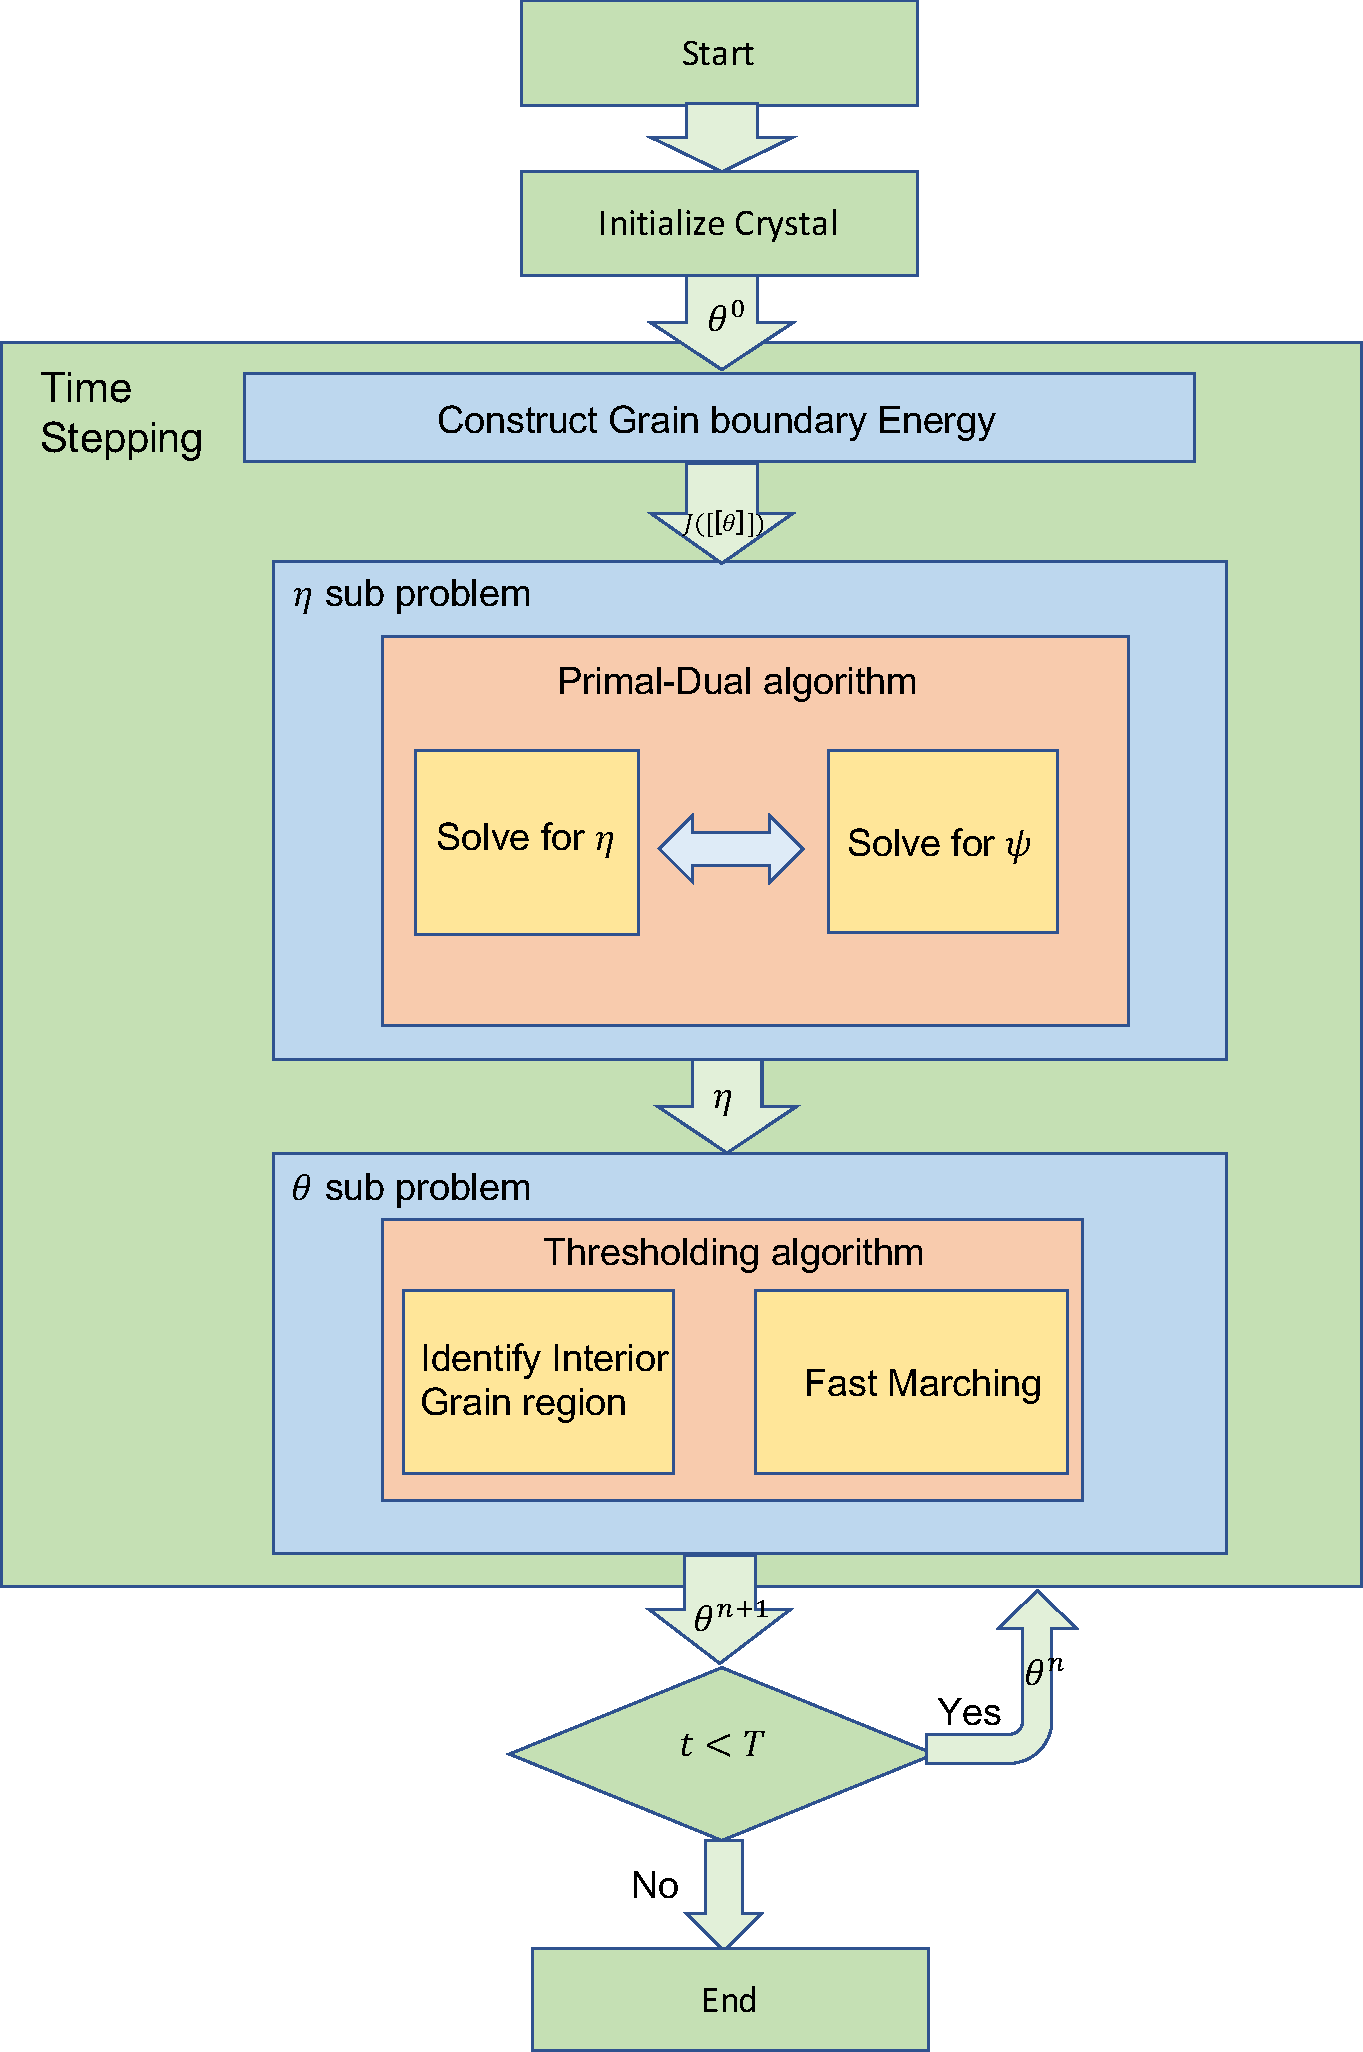
\includegraphics[width=0.7\textwidth]{Figures/flowChart.pdf}
\end{center}
\caption{Algorithm Flow chart}
\label{fig:flow_chart}
\end{figure}

The code is developed as $\texttt{C++}$ header-template library,
which a user can freely refer. 
\texttt{C++} Function \& Class are categorized into different header
files based on their task. 
These Functions \& Classes can be replaced by a user-defined form, 
as long as the input \& output format is consistent. 
See the list of header files in Table 1. 

To simulate an evolution of a polycrystal, a user first needs to define 
initial crystal on a regular rectangular domain.  
Several initial grain configuration 
such as bicrystal, tricrystal, and randomly distributed polycrystal
can be easily constructed using a function defined in \texttt{InitCrystal.h}.
Next, a user is required to define the jump function $\mathcal{J}\big( [\![\theta ]\!]\big)$.
The \texttt{Material} class defined in \texttt{Material.h} is useful for defining $\mathcal{J}$.
In the following, the \texttt{PrimalDual} class and 
\texttt{KWCThreshold} class should be constructed to
solve $\eta$-sub problem~(\ref{eqn:eta_sub}) and 
$\theta$-sub problem~(\ref{eqn:theta_sub}). 
After these classes are constructed, 
simulation will run until it reaches to a given final time. 
The flow chart of the overall algorithm is summarized 
in Figure~\ref{fig:flow_chart}. 



\begin{table}
\setstretch{1.2}
\begin{center}
\begin{tabular}{cc} \toprule
Header file     & Contents \\ \midrule
\texttt{InitCrystal.h} & Functions that set the initial condition of simulation, i.e. initialize $\theta(x)$\\
\texttt{DataOut.h} & Functions related to output solution for visualization\\
\texttt{Material.h} & A class that defines GB energy $\mathcal{J}\big( [\![ \theta ]\!] \big)$ of different types of material \\
\texttt{PostProcessor} & Functions that compute the KWC free energy of polycrystal\\
\texttt{PrimalDual.h} & A class that solves $\eta$-sub problem at a given $\theta(x)$ configuration\\
\texttt{KWCThresholding.h} & A class that solves $\theta$-sub problem at a given $\eta(x)$ configuration\\
\texttt{KWCJumpFunction.h} & A class that design $\mathcal{J}$ from a provided external GB data \\
\texttt{Metrics.h} & A list of simple mathematical functions
\end{tabular}
\caption{Table of header files}
\label{tab:symbols}
\end{center}
\end{table}


\section{An example: 2-D polycrystal simulation}

In this section, we will look into an example code file 
\texttt{KWC\_Polycrystal.cpp} in \texttt{E5} folder
and show how to execute this file.
This example code simulates grain boundary motion under 
given $\mathcal{J}\big( [\![ \theta ]\!] \big)$,
which is fitted against FCC [110] symmetric tilt grain boundary energy. 
Because this simulation includes the most of features of
the developed code, it will be helpful to understand 
how the steps in Fig.~\ref{fig:flow_chart} can be implemented 
using the template library. 


\subsection{Implementation file}

We will read the implementation code file block by block. 
A bullet point is used to emphasize the purpose of each block.  

\begin{itemize} \item First, we begin by listing the required header files \end{itemize}
\begin{tcolorbox}[breakable, enhanced]
\begin{lstlisting}[basicstyle=\footnotesize]
#include <stdlib.h>
#include <math.h>
#include <string.h>
#include <time.h>
#include <float.h>
#include <stdio.h>
#include <assert.h>
#include <iostream>
#include <vector>

//Relevant Library
#include "DataOut.h"
#include "InitCrystal.h"
#include "PostProcessor.h"
#include "PrimalDual.h"
#include "KWCThresholding.h"
\end{lstlisting}
\end{tcolorbox}

\begin{itemize} \item Then, in the \texttt{main} function, 
we define domain size. \end{itemize}

\begin{tcolorbox}[breakable, enhanced]
\begin{lstlisting}[basicstyle=\footnotesize]
int main(int argc, char *argv[]){

  //Read global variables from bash
  //Define grid size and set model parameter epsilon
  int n1=atoi(argv[1]);
  int n2=atoi(argv[2]);
  int n3=atoi(argv[3]);
  double epsilon=atof(argv[4]);

  int const DIM=3;
      
  //const unsigned int lcount=2;
  const unsigned int lcount=50;
    
  int pcount = n1*n2*n3;
  double dt= epsilon * epsilon; //initial choice of dt
	
  int Nthread = 1; //Number total thread to be used for FFTW	

\end{lstlisting}
\end{tcolorbox}

We will have to pass the domain size $N_x,N_y,N_z$
and the parameter $\epsilon$ 
from the command line when we execute the code. 
Also, note that in our thresholding scheme, 
the choice of $\epsilon$ determines the time step size $\delta t =\epsilon^2$.

\begin{itemize} \item We declare global variables \end{itemize}

\begin{tcolorbox}[breakable, enhanced]
\begin{lstlisting}[basicstyle=\footnotesize]
  double *Xangles = new double[lcount]();
  double *Yangles = new double[lcount]();
  double *Zangles = new double[lcount]();
  double *eta = new double[pcount]();
  int *labels = new int[pcount]();
  double *JField = new double[pcount]();
\end{lstlisting}
\end{tcolorbox}

We use pointer variables for these global variables 
and each independent \texttt{C++} class 
will communicate through their address. 


\begin{itemize} \item Then, we construct an initial polycrstal \end{itemize}

\begin{tcolorbox}[breakable, enhanced]
\begin{lstlisting}[basicstyle=\footnotesize]
  double maxZangle = 70.0* M_PI/180.0;
  InitializeCrystal::RandomCrystalConfiguration2D(n3,n2,n1,lcount,labels, 
         maxZangle, Xangles,Yangles,Zangles);
\end{lstlisting}
\end{tcolorbox}

This line will generate a randomly distributed 2-D polycrystal 
with the given maximum $Z$-orientaion value, using a voronoi tessellation.
Other crystal configurations can also 
be found in \texttt{InitCrystal.h} header file.
A user can also define new crystal configuration 
independently for one's own needs.  

\begin{itemize} \item Next, we construct a material class which calculates $\mathcal{J}$ \end{itemize}
 
\begin{tcolorbox}[breakable, enhanced]
\begin{lstlisting}[basicstyle=\footnotesize]
  char materialType='C';
  Material material(n3,n2,n1,materialType);

  //Designate the location of Jump function data
  if(materialType =='C')  {
    int dataNum=361;
    material.setCovarianceModel(dataNum, "inputs/jfun_cu_110.txt");
  }
\end{lstlisting}
\end{tcolorbox}
Here, we choose the material type 'C', which stands for the material,
of which grain boundary energy $\mathcal{J}$ is described by the 
covariance model~\cite{Runnels:2016_1,Runnels:2016_2}.
Then, we provide the information of $\mathcal{J}$ by
indicating the external data file.
On the other hand, if a use want to simulate the original KWC model, 
it can be done by simply designating the \texttt{materialType} as 'S'.

\begin{itemize} \item Construct numerical algorithm \texttt{C++} classes
and the link pointers of global variables \end{itemize}

\begin{tcolorbox}[breakable, enhanced]
\begin{lstlisting}[basicstyle=\footnotesize]
//Construct PD Algorithm class
double PDerror=1e-6; // tolerance of Primal-dual algorithm
int PDmaxIters=10000; // allowable iteration number of the algorithm

PrimalDual<DIM> EtaSubProblem(n3, n2, n1, PDerror, PDmaxIters,
				lcount,epsilon, Nthread);
  
//Link pointers of Global variables to the Primal-Dual algorithm class

EtaSubProblem.setUpClass(eta, Xangles, Yangles, Zangles,
labels, energyField,materialType);

double initThresCriteria = 2*epsilon ;
KWCThreshold<DIM> FastMarching(n3,n2,n1,lcount,initThresCriteria);
FastMarching.setUpClass(eta, Xangles, Yangles, Zangles, labels, JField,'P');
    
\end{lstlisting}
\end{tcolorbox}

Primal-dual class requires additional inputs for maximum allowable 
iteration counts and stopping criteria. 
Thresholding class requires the criteria for identifying the interior regions
of grains. The code will identify the interior grains where 
$\mathcal{J}\big( [\![ \theta]\!]\big) <$ \texttt{initThreCrietria}.

\begin{itemize} \item Now, we are finally ready to run the simulation \end{itemize}

\begin{tcolorbox}[breakable, enhanced]
\begin{lstlisting}[basicstyle=\footnotesize]
  for (int i =0 ; i<20 ; i++)
  {
    std::cout << "  " << i << "time-step begins...." << std::endl;
    
    material.calculateFieldJ('P');
    EtaSubProblem.run(epsilon);
    FastMarching.run(epsilon);
  }
\end{lstlisting}
\end{tcolorbox}


\begin{itemize} \item The final step is to release memory space \end{itemize}

\begin{tcolorbox}[breakable, enhanced]
\begin{lstlisting}[basicstyle=\footnotesize]

  EtaSubProblem.freeMemory();
  FastMarching.freeMemory();
  
  delete[] eta; eta=NULL;
  delete[] labels; labels=NULL;
  delete[] Xangles; Xangles=NULL;
  delete[] Yangles; Yangles=NULL;
  delete[] Zangles; Zangles=NULL;
\end{lstlisting}
\end{tcolorbox}

This is the end of \texttt{KWC\_Polycrystal.cpp}. 


\subsection{Environment and Execution}

In this section, we discuss required system environment 
and how to execute the code.
The developed code has been tested with 
and has been tested with a g++ compiler. 
Because the Primal-dual algorithm necessitates the use of 
Fast Fourier Transform (FFT) and inverse FFT,
we borrow relevant libraries from \texttt{FFTW3} library. 
We suggest to use a `makefile' tool to export these environment variables, 
an example format of which is as follow.\\

\begin{tcolorbox}[colback=white]
\begin{lstlisting}[basicstyle=\footnotesize]
IDIR  += -I../../include/KWC_Simulation

CC= g++
CFLAGS += -Ofast
CFLAGS += -std=c++14
CFLAGS += -lm
CFLAGS += -lfftw3_threads
CFLAGS += -lfftw3
program: 
	$(CC) KWC_polycrystal.cpp -o main $(CFLAGS) $(IDIR)
\end{lstlisting}
\end{tcolorbox}

For data visualization options, 
we use \texttt{ffmpeg} libraries and \texttt{Paraview}. 
Yet, those two softwares are not mandatory. \\

Once the implementation code file \texttt{KWC\_Polycrystal.cpp} 
is successfully compiled, it will create an executable, 
say that it is `main'. The executable can be run with following arguments, 
which stands for size of computational domain $N_x,N_y,N_z$, 
and $\epsilon$ value. 
 
\begin{tcolorbox}[colback=white]
\begin{lstlisting}[basicstyle=\footnotesize]
./main 512 512 1 0.05
\end{lstlisting}
\end{tcolorbox}

\section{Data structure}

In this section, we summarize how data is being stored in the current code 
and recommend useful built-in \texttt{C++} functions that visualizes this data. 
Understanding the data structure and knowing how to quickly visualize
will be useful, when a user wants to modify or build something more 
on the current library for one's own purpose. 


\subsection{Discrete field data stored in one dimensional array}
Any discrete scalar field data (either 2D or 3D) in this library is saved in one dimensional array. 
The index of the array first increases in $x$ direction, then $y$ and $z$ direction. 
In a regular square domain, the discrete field, say $\eta(x,y,z)$, can be assessed as 

\begin{tcolorbox}[breakable, enhanced]
\begin{lstlisting}[basicstyle=\footnotesize]
  /* Example: assess eta(x,y,z) and save it to Pvalue */

  double Pvlalue;
 
  for(int i=0; i<n3; i++)  { // z loop
    for(int j=0; j<n2; j++)  { //y loop
      for(int k=0; k<n1; k++)  { //x loop
        
        double x = k/n1
        double y = j/n2
        double z = i/n3;
 
        Pvalue= eta[i*n2*n1+j*n1+k]; 
      }
     }
  }
\end{lstlisting}
\end{tcolorbox}

The only exception is the orientation field $\theta$.
In case of $\theta$, we save \texttt{int-type} labels at each grid point
and each component of orientation values corresponding to the label is saved separately. 
For example, the $\theta$ value in $Z$-direction at point $(x,y,z)$ 
can be assessed as follow
\begin{tcolorbox}[breakable, enhanced]
\begin{lstlisting}[basicstyle=\footnotesize]
  /* Example: assess theta_Z (x,y,z) and save it to Ztheta */

  double Ztheta;
 
  for(int i=0; i<n3; i++)  { // z loop
    for(int j=0; j<n2; j++)  { //y loop
      for(int k=0; k<n1; k++)  { //x loop
        
        Ztheta= Zangles[labels[i*n1*n2+j*n1+k]] 
      }
     }
  }
\end{lstlisting}
\end{tcolorbox}

\subsection{Output data in vtu format}

\texttt{C++} functions defined in \texttt{DataOut.h} can be useful 
to visualize results in a format that many visualization software (e.g. \texttt{Paraview}) 
can read. Any scalar field data in 2D in the above data structure (one dimensional array)
and orientation field data can be simply output to \texttt{.vtu} as follow 

\begin{tcolorbox}[breakable, enhanced]
\begin{lstlisting}[basicstyle=\footnotesize]
  /* Example: Output eta and output to the file  "myeta_0.vtu" */
Output2DvtuScalar(n1, n2, n3, eta, "eta value", "myfile_",0);

 /* Example: Output Z_theta and output to the file  "mytheta_0.vtu" */
Output2DvtuAngle(n1, n2, n3, Zangles, labels, "theta_Z", "myfile_",0); 
\end{lstlisting}
\end{tcolorbox}


\section{Additional Features}

This section is devoted to introduce 
additional features of the developed code
that has not been included in the previous example code. 

%%Work from here!!
\subsection{Design of the jump function}

The example code \texttt{Design\_J.cpp} in the \texttt{E4} folder 
uses a Newton's iteration 
to fit $\mathcal{J}\big( [\![ \theta]\!]\big)$ to an external grain boundary energy data. 
The code takes an input file \texttt{STGB\_cu\_110.txt} which is 
the covariance model prediction of FCC [110] Symmetric-tilt-grain-boundary energy~\cite{Runnels:2016_1,Runnels:2016_2}. 
The format of the input file is as follow\\

\begin{tcolorbox}[colback=white]
\begin{lstlisting}[basicstyle=\footnotesize]
 # tiltAngle(deg)         # W_data
 # ------------            -------------  
                   0        	     0.0
                 0.5             0.10458
                   1            0.203463
                 1.5            0.296963
                   2            0.385376
                 2.5            0.468977
                   3            0.548028
                 3.5            0.598243
... (continues)
\end{lstlisting}
\end{tcolorbox}       

To construct $\mathcal{J}$, we can call \texttt{KWCDesignJ} \texttt{C++ class}.
We only need to provide the number of data and the name of input\&output file as follow.\\

\begin{tcolorbox}[breakable, enhanced]
\begin{lstlisting}[basicstyle=\footnotesize]
int main(int argc, const char * argv[]) {
     int nData=361;
     KWCDesignJ optimizer(nData,"STGB_cu_110.txt","J_cu_110.txt");
     optimizer.run(); 
     return 0;
}
\end{lstlisting}
\end{tcolorbox}


Then, the output file format, \texttt{J\_cu\_110.txt} can be later used for grain growth simulation.\\
\begin{tcolorbox}[colback=white]
\begin{lstlisting}[basicstyle=\footnotesize]
    # tiltAngle       # Jtheta # Total Energy
 # ------------  -------------   -------------
              0              0              0
            0.5      0.0432744        0.10458
              1       0.102464       0.203463
            1.5       0.171975       0.296963
              2       0.250429       0.385376
            2.5       0.337459       0.468977
              3       0.433323       0.548028
            3.5       0.502413       0.598243
... (continues)
\end{lstlisting}
\end{tcolorbox}

\subsection{Setting FFMEPG for evolving grain animation}


The developed code can generate grain evolution movie while simulation is running.
This necessitates that \texttt{ffmpeg} be installed on the machine. 
We will convert the Z-orientation value of grains into a number between 
[0,255]. Then, we will use black-and-white images to collect pictures of grains 
at each time step. 
To do this, we need to prepare it as follow 
\\

\begin{tcolorbox}[breakable, enhanced]
\begin{lstlisting}[basicstyle=\footnotesize]
  /* movie data */
  unsigned char *pixels=new unsigned char[pcount];
  
  unsigned char *colors=new unsigned char[lcount];
  for(int l=0;l<lcount;l++){
      // Distribute colors to angles
        colors[l]=255*Zangles[l]/maxZangle;
  }
  
  char *string;
  asprintf(&string,"ffmpeg -y -f rawvideo -vcodec rawvideo -pix_fmt gray -s 
   %dx%d -r 30 -i - -f mp4 -q:v 5 -an -vcodec mpeg4 out.mp4", n1,n2);
  
  //open an output pipe
  FILE *pipeout = popen(string, "w");
  
\end{lstlisting}
\end{tcolorbox}
Then, we use ``\texttt{PrepareFFMPEG2DPixel}" function defined it
\texttt{DataOut.h} to convert orientation data to image

\begin{tcolorbox}[breakable, enhanced]
\begin{lstlisting}[basicstyle=\footnotesize]
  for (int i =0 ; i<20 ; i++)
  {
    std::cout << "  " << i << "time-step begins...." << std::endl;
    PrepareFFMPEG2DPixels(n1,n2,0,pixels, labels, colors);
    fwrite(pixels, 1, pcount, pipeout);
    material.calculateFieldJ('P');
    EtaSubProblem.run(epsilon);
    FastMarching.run(epsilon);
  }
\end{lstlisting}
\end{tcolorbox}




\newpage

%\begin{itemize} \item Run simulation \end{itemize}
%We take 200 time steps, and the pixel grain data will be 
%reformatted to black-and-white image data. \\
%\begin{tcolorbox}[breakable, enhanced]
%\begin{lstlisting}[basicstyle=\footnotesize]
%  //Start Dynamics
%  for (int i =0 ; i<200 ; i++)
%  {
%    PrepareFFMPEG2DPixels(n1,n2,0,pixels, labels, colors);
%    fwrite(pixels, 1, pcount, pipeout);
%      
%    EtaSubProblem.run(material, epsilon);
%    FastMarching.run(epsilon);
%  }
%\end{lstlisting}
%\end{tcolorbox}
%
%\section{Additional features}
%
%The main advantage of using the alternate KWC model is
%that one can freely construct the function $\mathcal{J}$ in Eq~(\ref{eqn:alternateKWC}).
%In this example, we will how to use alternate simulation. 
% 
%\subsubsection{Design the jump function}
%
%The example code \texttt{Design\_J.cpp} uses a Newton's iteration 
%to fit $\mathcal{J}\big( [\![ \theta]\!]\big)$ to an external grain boundary energy data. 
%The code takes an input file \texttt{STGB\_cu\_110.txt} which is 
%the covariance model prediction of FCC [110] Symmetric-tilt-grain-boundary energy~\cite{Runnels:2016_1,Runnels:2016_2}. 
%The format of the input file is as follow\\
%
%\begin{tcolorbox}[colback=white]
%\begin{lstlisting}[basicstyle=\footnotesize]
% # tiltAngle(deg)         # W_data
% # ------------            -------------  
%                   0        	     0.0
%                 0.5             0.10458
%                   1            0.203463
%                 1.5            0.296963
%                   2            0.385376
%                 2.5            0.468977
%                   3            0.548028
%                 3.5            0.598243
%... (continues)
%\end{lstlisting}
%\end{tcolorbox}       
%
%To construct $\mathcal{J}$, we can call \texttt{KWCDesignJ} \texttt{C++ class}.
%We only need to provide the number of data and the name of input\&output file as follow.\\
%
%\begin{tcolorbox}[breakable, enhanced]
%\begin{lstlisting}[basicstyle=\footnotesize]
%int main(int argc, const char * argv[]) {
%     int nData=361;
%     KWCDesignJ optimizer(nData,"STGB_cu_110.txt","J_cu_110.txt");
%     optimizer.run(); 
%     return 0;
%}
%\end{lstlisting}
%\end{tcolorbox}
%
%
%Then, the output file format, \texttt{J\_cu\_110.txt} can be later used for grain growth simulation.\\
%\begin{tcolorbox}[colback=white]
%\begin{lstlisting}[basicstyle=\footnotesize]
%    # tiltAngle       # Jtheta # Total Energy
% # ------------  -------------   -------------
%              0              0              0
%            0.5      0.0432744        0.10458
%              1       0.102464       0.203463
%            1.5       0.171975       0.296963
%              2       0.250429       0.385376
%            2.5       0.337459       0.468977
%              3       0.433323       0.548028
%            3.5       0.502413       0.598243
%... (continues)
%\end{lstlisting}
%\end{tcolorbox}      
%
%\subsection{Running KWC polycrystal simulation with the designed J}
%
%Now, we are ready to simulate grain evolution 
%with crystal symmetry-invariance grain boundary energy. 
%Most of program structure is same with the previous polycrystal simulation code, 
%but we only need to simply replace the material type as `c' and designate 
%the $\mathcal{J}$ data.\\
%
%\begin{itemize} \item Set material types\end{itemize}
%
%\begin{tcolorbox}[breakable, enhanced]
%\begin{lstlisting}[basicstyle=\footnotesize]
%char materialType='c';
%  Material material;
%
%  if(materialType =='c')  {
%    material.setCovarianceModel(361, "inputs/jfun_cu_110.txt");
%  }
%\end{lstlisting}
%\end{tcolorbox}
%
%
%
%
%\section{Environment}
%The current code is written by \texttt{C++} language 
%and has been tested with g++ compiler. 
%For Fast Fourier Transform (FFT) and inverse FFT, 
%it borrows necessary operators from  \texttt{FFTW3} library. 
%Simple linear algebra is operated through a \texttt{Eigen} software. 
%We suggest to use a `makefile' tool to export these environment variables, 
%an example format of which is as follow
%\begin{tcolorbox}[colback=white]
%\begin{lstlisting}[basicstyle=\footnotesize]
%IDIR  += -I../../include/KWC_Simulation
%IDIR  += -I../../Eigen
%CC= g++
%CFLAGS += -Ofast
%CFLAGS += -std=c++14
%CFLAGS += -lm
%CFLAGS += -lfftw3_threads
%CFLAGS += -lfftw3
%program: 
%	$(CC) KWC_driver.cpp -o main $(CFLAGS) $(IDIR)
%\end{lstlisting}
%\end{tcolorbox}
%For data visualization, we use \texttt{ffmpeg} libraries and \texttt{Paraview}. 
%Yet, those two are not mandatory.  
%
%
%
%\subsection{Compile and Execution}
%
%Once an implementation code \texttt{.cpp} 
%is successfully compiled, it will create an executable, 
%Say that it is `main'. The executable can be run with following arguments, 
%which stands for size of computational domain $N_x,N_y,N_z$, 
%and $\epsilon$ value. 
% 
%\begin{tcolorbox}[colback=white]
%\begin{lstlisting}[basicstyle=\footnotesize]
%./main 512 512 1 0.05
%\end{lstlisting}
%\end{tcolorbox}


\bibliographystyle{unsrt}
\bibliography{references}



%%Begin Algorithm Alternate KWC simulation
%\begin{algorithm}
%    \setstretch{1.1}\small
%    \SetKwInOut{Input}{Input} % For compile
%    \SetKwInOut{Output}{Output} % For compile
%    \Input{System size $N$, parameter $\epsilon,\xi$ and  an initial grain configuration $\theta^{0}$}
%    \Output{Time evolution of the alternate KWC model} 
%    
%    Initialize Grains $\theta^{0}$ on domain $\Omega$\\
%    \While{ t $<$ T} {
%    Compute grain boundary energy $\mathcal{J} \big( [\![ \theta ]\!] \big)$\\
%    
%    \hfill\linebreak     
%    \CommentSty{Execute Primal-dual algorithm}\\
%    
%     \While{$\mathrm{max}(\eta^{n+1}-\eta^{n})< tol$}
%    {
%    Update $\eta^{n+1}$ using $\psi^{n}$  
%    Update $\psi^{n+1}$ using $\eta^{n+1}$  
%    }
%     
%    \hfill\linebreak    
%    \CommentSty{Execute thresholding algorithm}\\
%    
%    Identify interior regions of grains $I_p$ 
%    
%    \quad\quad  \CommentSty{Execute Fast Marching}\\
%    \quad\quad Allow each grain $I_p$ to grow with speed $1/(1-\eta)^2$\\
%    \quad\quad Threshold $\theta(x), x\in \Omega-I$ to that of a interior grain arrives at earliest  
%     
%    \hfill\linebreak
%    Compute free energy $\mathcal{W}_{\mathrm{kwc}}(\eta,\theta)$\\
%
%    } %End of time (t<T) while
%    \caption{Suggested algorithms for the alternative KWC simulation}
%    \label{algorithm:KWC}
%\end{algorithm}
%%% End algorithm 



\end{document}
